\scanpage{501}
\mspage{254}

thus by $(*)$ we have $u(l_i)\in L_i$ i.e. $u(L_i)\subset L_i$,
but we have $\operatorname{Aut}(L_i)\simeq\widehat{\mathbb Z}^{*}$, and an
\unsure{endomorphism|automorphism} \unsure{of the|of a} \deleted{\unsure{$L_i$}}
$\widehat{\mathbb Z}$-\unsure{module|modules} \unsure{free|free} of rank $1$
\inserted{$L_i$} is known when one knows it
on an $nL_i\xleftarrow{\sim}L_i$.
Thus \inserted{$\forall i$ \unsure{we have}} $u(l_i)=l_i$,
thus $u=\mathrm{id}$, q.e.d.

In the case where $\pi$ is not free,
take a \deleted{system of} basis $(x_i,y_i)_{1\leq i\leq g}$
-- so that $\pi$ is defined by the generating relation
\[
\tag{3} \prod_1^g[x_i,y_i]=1,
\]
let $\Lambda_i$, $\Lambda'_i$ be the closed subgroups
generated by $x_i,y_i$.
\deleted{I admit} (They are moreover all conjugate under
$\operatorname{Aut}(\pi)$\ldots) I admit that these groups
are $\simeq\widehat{\mathbb Z}$ (i.e. that the
\inserted{surjective} homomorphisms $\widehat{\mathbb Z}\longrightarrow\Lambda_i$,
$\widehat{\mathbb Z}\longrightarrow\Lambda'_i$ sending $1$ to the
$x_i,y_i$ are injective -- this \deleted{\unsure{should not be hard}}
\inserted{this is moreover trivial} on passing to $\pi_{\mathrm{ab}}$)
\uline{and} that we have, by analogy with (2), for
every $n\in\unsure{\mathbb N^{*}}$
\[
\tag{4}
\operatorname{Centr}_{\pi}(\Lambda_i^n)=\Lambda_i,\qquad
\operatorname{Centr}_{\pi}(\Lambda_i'{}^n)=\Lambda'_i,
\]

\scanpage{502}

and we finish as above.

\uline{Remark} The strongest faithfulness
result in the direction of the present
\S, concerning actions of $\mathbb{\Gamma}$ and of
its open subgroups, would be the
following: if $\unsure{V}$ is an
anabelian algebraic curve over the finite
extension $k$ of $\mathbb Q$, with the algebraic closure $\bar k$,
then not only should the outer action
of $\mathcal E_k^{\bar k}=\Gamma$ on
$\pi_1(\unsure{V}_{\bar k})$ be
faithful, i.e.
\[
\Gamma\longrightarrow\unsure{\widehat{\widehat{\mathcal T}}}(\pi)
\]
\margin{this \unsure{homomorphism$^{\mathrm m}$} \unsure{is} \unsure{automatically factored}
through the subgroup $\mathcal N(\pi)$ which \unsure{interests us \illegible{1}|normalizes}
$\widehat{\mathcal T}(\pi)$}
injective, but even the composite
homomorphism
\[
\Gamma\longrightarrow
\unsure{\mathcal N_4(\pi)|\mathcal N_{\Delta}(\pi)}
\longrightarrow\mathcal N(\pi)/\widehat{\mathcal T}^{+}(\pi)
\simeq\mathbb{\Gamma}_{\pi}
\]
should be injective (in which case it will
even be an isomorphism, since it is
surjective by the very construction of
$\mathcal N(\pi),\mathbb{\Gamma}_{\pi}$\ldots)
Some heuris-

\scanpage{503}
\mspage{255}

tic arguments made previously (probably less convincing than those of the present
\S~!) seem to indicate that this would be
the case at least when $V$ is an
étale covering of $U=(U_{03})_k$, in which
case indeed the homomorphism $\Gamma\longrightarrow\mathbb{\Gamma}_{\pi}$
fits into a commutative diagram
\diagram{\begin{tikzcd}[ampersand replacement=\&,column sep=large,row sep=large]
\& \Gamma \arrow[dl] \arrow[d] \arrow[dr] \& \\
\mathbb{\Gamma}_{\pi_0}
 \arrow[rr,bend right=23]
 \arrow[rr,bend left=20,phantom,"{\deleted{\unsure{\longrightarrow}}}" description]
\& \mathbb{\Gamma}_{\pi} \arrow[r] \& \mathbb{\Gamma}_{\pi'}
\end{tikzcd}}
where $\pi_0=\pi(U_{\bar k})$, so that $\pi$ is an open subgroup of
$\pi_0$, and $\unsure{\pi''|\pi'}$ is a
suitable open subgroup, \uline{characteristic}
in $\pi_0$. \uline{\uuline{If}} we could show that
$\mathbb{\Gamma}_{\pi_0}\longrightarrow\mathbb{\Gamma}_{\pi'}$ is injective
(which is $\pm$ a matter of profinite algebra), this would
likewise be true of the composite
$\Gamma\unsure{\hookrightarrow|\subset}\mathbb{\Gamma}_{\pi_0}
\longrightarrow\mathbb{\Gamma}_{\pi'}$,
thus also of $\Gamma\longrightarrow\mathbb{\Gamma}_{\pi}$.
Thus modulo this hypothesis on profinite groups,
and using \unsure{Belyi}, we find that

\scanpage{504}
for every algebraic curve $V$ over $k$,
$\exists\ V'\subset V$ nonempty open, such that
\[
\Gamma\longrightarrow\mathbb{\Gamma}_{\pi'}
\qquad (\text{where }\pi'=\pi_1(V'_{\bar{k}}))
\]
is injective. As for knowing whether
$\Gamma\longrightarrow\mathbb{\Gamma}_{\pi}$ is itself already injective
-- or \deleted{\illegible{1}} what amounts to the same thing, whether
$\Gamma\longrightarrow\mathbb{\Gamma}_g$ for $g\geq 2$, and
$\Gamma\longrightarrow\mathbb{\Gamma}_{1,1}$ are injective,
I have no plausible heuristic reason to convince me of it at present
-- \unsure{perhaps|may be} this is entirely false ? The
more or less convincing argument \unsure{recalled} previously (assuming we
\unsure{manage} to justify it) \unsure{would show} only that if
$\Gamma\longrightarrow\mathbb{\Gamma}_{\pi}$ is injective for
\uline{one} $\pi$ (which depends only on \unsure{its} type $(g,\nu)$)
then it is so for the $\pi'$ open in $\pi$.
\deleted{But is \unsure{it|-it} true that} \inserted{We know it at}

\scanpage{505}
\mspage{256}
present (modulo very little, at any rate)
for the types $(0,\nu)$ $(\nu\geq 3)$ exactly
-- no more, no less -- and we could
perhaps deduce it for types $(g,\nu)$
which are deduced from them by ``finite \unsure{covering}''.
But it is already clear that we do not obtain
the types $(g,0)$ in this way $(g\geq 2)$,
nor even any $(g,\nu)$ with $g\geq 1$, $\nu\in\{0,1,2\}$\unsure{.|-}
That is to say we are far from the mark\ldots
The first really interesting case would
thus be the case $(1\unsure{,}1)$, where
$\widehat{\mathcal{T}}_{1,1}^{+}\simeq
\unsure{\mathrm{Sl}|\mathrm{SL}}(2,\mathbb{Z})^{\wedge}$
\margin{torus with one hole !}
\unsure{Operating|operating} by outer automorphisms on $\widehat{\Pi}_{1,1}$
(a free group on two generators, again
-- as if by chance) -- is the
``arithmetic'' action of $\mathbb{\Gamma}_{\mathbb{Q}}$ on $\widehat{\Pi}_{1,1}$
(i.e. the outer action \uline{modulo}
\inserted{$\widehat{\mathcal{T}}_{1,1}^{+}\simeq$}
$\unsure{\mathrm{Sl}|\mathrm{SL}}(2,\mathbb{Z})^{\wedge}$)
faithful ?

\scanpage{506}
\mspage{257}
\uline{36} The isomorphism
$\mathbb{\Gamma}_{\mathbb{Q}}\xrightarrow{\sim}\mathbb{\Gamma}_{1,1}$,
and the injectivity of
$\mathbb{\Gamma}_{\mathbb{Q}}\longrightarrow
\mathrm{Aut\,ext}_{\unsure{\mathrm{lac}}}(\widehat{\mathcal{T}}_{11}^{+})
\simeq\mathrm{Aut\,ext}_{\unsure{\mathrm{lac}}}(\unsure{\mathrm{Sl}|\mathrm{SL}}(2,\mathbb{Z})^{\wedge})$
\margin{The \unsure{reflections|reflections} of the present \S,
a bit halting, will be taken up again in a \unsure{way|way}
less ponderous in the \S\ that follows\ldots}

Let $\Pi'_{03}$ be the quotient group of $\Pi_{03}$
\unsure{defined} by \unsure{\uline{the}} relations
\[
(1)\qquad l_1^2=l_\infty^3=1
\]
-- this is therefore the ``oriented cartographic
group \inserted{for triangulated structures}''\unsure{,|;}
\deleted{whose} the finite $\Pi'_{0,3}$-sets
\deleted{on which} \unsure{correspond|corresponding} to
\unsure{oriented} \unsure{finite} maps (\unsure{possibly} having
flattened loops) whose faces are
triangles or mono-angles. The outer
operation of $\mathbb{\Gamma}_{\mathbb{Q}}$
(but not that of $\unsure{\mathfrak{S}_3|\mathcal{S}_3}$ !)
on $\widehat{\Pi}_{03}$ passes to the quotient as an
action on $\widehat{\Pi}'_{0,3}$. We can improve
\unsure{theorem} 1 of the preceding \S\ by \unsure{the|the}

\uline{Proposition} The outer action of $\mathbb{\Gamma}_{\mathbb{Q}}$
on $\widehat{\Pi}'_{0,3}$ is faithful.
\figure{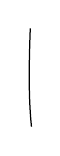
\begin{tikzpicture}[x=1cm,y=1cm]
\draw[line width=.45pt] (0,1.25) .. controls (-.015,.82) and (-.025,.40) .. (.015,0);
\end{tikzpicture}}

To show this, we shall embed
$\Pi_{0,3}$ as a subgroup of finite index
in $\Pi'_{0,3}$, whence an \unsure{analogous} embedding
\deleted{\illegible{1}}
\[
(2)\qquad\widehat{\Pi}_{0,3}\lhook\joinrel\longrightarrow\widehat{\Pi}'_{0,3}
\]
which will be compatible with the outer action of $\Gamma$.

\scanpage{507}

For this, consider the quotient scheme
\[
Y=\underbrace{\mathbb P^1_{\mathbb Q}}_{X}/\unsure{\mathfrak S_3}
\]
with the three points \inserted{$a_0,a_1,a_\infty$} of $Y$, rational over
$\mathbb Q$, \inserted{$a_0$} corresponding to the orbit
\deleted{of the} $\{0,1,\infty\}$, $a_1$ to the orbit
$\{-1,\frac12,2\}$, and $a_\infty$ to the orbit
$\{\unsure{-j},\unsure{-\overline j}\}$ of $\unsure{\mathfrak S_3}$
\margin{$j=\exp\frac{2i\pi}{3}$}
(which exhausts \unsure{the set} of geometric
``singular'' orbits). We know that $Y$ is a projective line
(over $\overline{\mathbb Q}$ a priori), \unsure{which we} \unsure{pin} by
$a_0,a_1,a_\infty$ as points $0,1,\infty$, \unsure{(thus}
$Y\simeq\mathbb P^1_{\mathbb Q}$ -- the \deleted{\illegible{1}} morphism
$X\longrightarrow Y$ is thus identified with a well-determined morphism
\[
(3)\qquad
f:\begin{array}{ccc}
\mathbb P^1_{\mathbb Q}&\longrightarrow&\mathbb P^1_{\mathbb Q}\\
\Vert&&\Vert\\
X&&Y
\end{array}
\]
\deleted{(in fact, $f$ can be defined as a morphism
$\mathbb P^1_{\mathbb Z}\longrightarrow\mathbb P^1_{\mathbb Z}$,
but here this matters little to us)}
which makes $X$ a Galois \unsure{covering|covering} of $Y$, with group
$\unsure{\mathfrak S_3}$, étale \unsure{over|over}
$\mathbb P^1_{\mathbb Q}\setminus\{0,1,\infty\}$, with ramification
indices at these points $2,2,3$. From the point of view of the geometry of maps
(\unsure{placing oneself|immersing oneself} over the base field $\mathbb C$), we consider the

\scanpage{508}
\mspage{\unsure{258 (259)}}

map determined on $X$ by the spherical triangles $(0,1,\infty)$
(on the real axis as equator) -- which is thus the universal
\unsure{weighted} triangular map -- as the inverse image of the universal map
(having a single vertex $0$, a single edge (folded) $0\longrightarrow1$,
a single face, with center $\infty$).
\margin{\figure{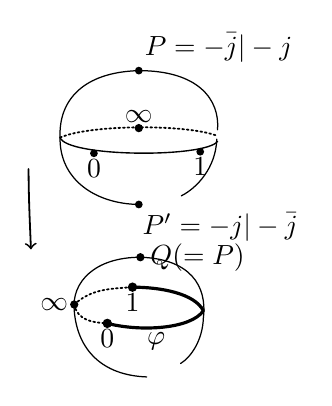
\begin{tikzpicture}[x=1cm,y=1cm,line cap=round,line join=round]
\draw[line width=.45pt] (0,2.85)
 .. controls (-.71,2.83) and (-1.02,2.47) .. (-1,2)
 .. controls (-1.01,1.48) and (-.57,1.16) .. (0,1.15);
\draw[line width=.45pt] (0,2.85)
 .. controls (.76,2.85) and (1.03,2.48) .. (1,2.10);
\draw[line width=.45pt] (.99,1.98)
 .. controls (.98,1.62) and (.74,1.36) .. (.54,1.26);
\draw[line width=.5pt] (-1,2)
 .. controls (-.91,1.75) and (.83,1.74) .. (1,1.95);
\draw[densely dotted,line width=.65pt] (-1,2)
 .. controls (-.61,2.17) and (.63,2.17) .. (1,2.02);
\fill (0,2.85) circle (1.4pt);
\node[anchor=south west,inner sep=2pt] at (0,2.88) {$P=\unsure{-\bar j|-j}$};
\fill (0,1.15) circle (1.4pt);
\node[anchor=north west,inner sep=2pt] at (-.03,1.12) {$P'=\unsure{-j|-\bar j}$};
\fill (-.57,1.80) circle (1.4pt);
\node[below,inner sep=2pt] at (-.57,1.80) {$0$};
\fill (.78,1.82) circle (1.4pt);
\node[below,inner sep=2pt] at (.78,1.82) {$1$};
\fill (0,2.12) circle (1.5pt);
\node[above,inner sep=2pt] at (0,2.12) {$\infty$};
\draw[->,line width=.65pt] (-1.40,1.60)
 .. controls (-1.40,1.22) and (-1.38,.85) .. (-1.37,.58);
\draw[line width=.45pt] (.02,.48)
 .. controls (-.55,.48) and (-.86,.17) .. (-.82,-.20)
 .. controls (-.78,-.70) and (-.46,-1.02) .. (.10,-1.04);
\draw[line width=.45pt] (.02,.48)
 .. controls (.65,.46) and (.87,.12) .. (.82,-.29)
 .. controls (.81,-.58) and (.66,-.79) .. (.53,-.87);
\fill (.02,.48) circle (1.5pt);
\node[anchor=west,inner sep=2pt] at (.07,.48) {$\unsure{Q}(=P)$};
\fill (-.82,-.12) circle (1.5pt);
\node[left,inner sep=2pt] at (-.82,-.12) {$\infty$};
\fill (-.08,.10) circle (1.7pt);
\node[below,inner sep=2pt] at (-.08,.10) {$1$};
\fill (-.40,-.36) circle (1.7pt);
\node[below,inner sep=2pt] at (-.40,-.36) {$0$};
\draw[line width=1.15pt] (-.08,.10)
 .. controls (.28,.10) and (.71,.02) .. (.82,-.20)
 .. controls (.66,-.43) and (.03,-.47) .. (-.40,-.36);
\draw[densely dotted,line width=.65pt] (-.82,-.12)
 .. controls (-.60,.08) and (-.36,.08) .. (-.08,.10);
\draw[densely dotted,line width=.65pt] (-.82,-.12)
 .. controls (-.78,-.32) and (-.59,-.35) .. (-.40,-.36);
\node[below,inner sep=1pt] at (.22,-.44) {$\unsure{\varphi}$};
\end{tikzpicture}}}
Every topological \deleted{\unsure{of}} \inserted{étale} covering of
$U_{03}(\mathbb C)\subset X$ thus gives a topological étale covering of
$U_{0,3}(\mathbb C)\subset Y$, \deleted{ramified} having
\deleted{\illegible{1}} \inserted{over} $1$ ramification $2$,
over $\infty$ ramification $3$ \unsure{exactly|exactly},
which corresponds to the ``forgetful'' functor \inserted{(of the weighting)},
where a \unsure{weighted} triangular map is considered as
just a map. From the point of view of fundamental groups \unsure{we} thus find
an \deleted{\unsure{homomorphism} of outer groups}
\inserted{equivalence of categories}

\diagram{\begin{tikzcd}[ampersand replacement=\&,column sep=large,row sep=huge]
\&
\deleted{\begin{gathered}
\Pi_1(\unsure{X(\mathbb C)}\setminus\{0,1,\infty\})\\[-2pt]
\rotatebox{90}{$=$}\\[-2pt]
\Pi_{0,3}
\end{gathered}}
\arrow[r,phantom,"{\deleted{\longleftarrow}}" description]
\&
\deleted{\begin{gathered}
\Pi_1\!\left(Y(\mathbb C)\setminus\{0,1,\infty\};
\underbrace{2\{1\}+3\{\infty\}}_{\substack{\text{signature of}\\\text{ramification}}}\right)\\[-2pt]
\rotatebox{90}{$=$}\\[-2pt]
\Pi'_{0,3}
\end{gathered}}
\\
(\deleted{\illegible{1}}\inserted{4}) \&
\left(\text{Étale coverings of }X\setminus\{0,1,\infty\}=U_{0,3}\right)
\arrow[r,phantom,"\simeq" description]
\arrow[d,phantom,"{\rotatebox{-90}{$\simeq$}}" description]
\&
\begin{gathered}
\left[\begin{gathered}
\text{Coverings of }Y\setminus\{0,1,\infty\}=U_{0,3}\\
\text{with ramification subordinate to}\\
\text{the signature }2\{1\}+3\{\infty\}
\end{gathered}\right]\\
\big/\begin{gathered}
\text{the object }(X\setminus\{0,1,\infty\})\\
\text{of the said category}
\end{gathered}
\end{gathered}
\arrow[d,phantom,"{\rotatebox{90}{$\simeq$}}" description]
\\
\& \Pi_{0,3}\text{-sets} \&
(\Pi'_{0,3}\text{-Sets})/\deleted{\unsure{E}}E
\end{tikzcd}}

where $E$ is the $\Pi'_{0,3}$-set corresponding to the object
$X\setminus\{0,1,\infty\}$ of the category of étale coverings of
$\unsure{Y\setminus\{0,1,\infty\}}$ with ramification
\deleted{\unsure{imposed}}\inserted{\unsure{subordin-}}ate to
$2\{1\}+3\{\infty\}$

\deleted{$\unsure{\simeq}\ \unsure{\Pi_{0,3}^{\prime\circ}}\in\mathrm{Ens}$}

\scanpage{509}
\mspage{\unsure{260|250}}

Here, \deleted{\illegible{3}} \inserted{\deleted{\illegible{1}} the base point of $Y-\{0,1,\infty\}$ chosen\unsure{;|,} \unsure{to} describe the} coverings \deleted{$E=\unsure{f^{-1}}\unsure{(}$} (with ramification \unsure{subordinate} to \dots) by a fundamental group with ramification, being \unsure{again} $P=-\bar j$, we shall have
\[
(5)\qquad E=f_{\unsure{\mathbf C|\mathbb C}}^{-1}(P)
\]
and we can thus make explicit the category $(\Pi'_{03}\text{-Sets})/E$\unsure{;}

Where $E$ is a homogeneous space, \inserted{\unsure{isomorphic to the}} \unsure{quotient} of $\Pi'_{03}$ by the \unsure{subgroup|subgroup} \inserted{$\Pi'^{\circ}_{03}$} kernel of the \inserted{suitable} surjective homomorphism
\[
(6)\qquad
\left\{
\begin{array}{l}
\Pi'_{0,3}\longrightarrow\unsure{\mathfrak S_3|\mathcal S_3}\\[2pt]
\left.
\begin{array}{lll}
\ell_0 &\longmapsto& \text{element of order 2}\\
\ell_1 &\longmapsto& \text{element of order 2}\\
\ell_\infty &\longmapsto& \text{\unsure{element} of order 3}
\end{array}
\right)\quad\text{to be computed !}
\end{array}
\right.
\]

We choose a $Q_0\in E$ as ``origin'' of $E$ -- so as to be able to identify $E$ as a $\Pi'_{0,3}$-set with $\Pi'_{03}/\Pi'^{\circ}_{03}\simeq\unsure{\mathfrak S_3}$ -- then $(\mathrm{Ens}\,\Pi'_{03})/E$ is identified, by the functor $F\longmapsto F_{Q_0}$, with $\mathrm{Ens}(\Pi'^{\circ}_{03})$.

We thus find in summary an equivalence of categories (depending on the choice of $Q_0$)
\[
\Pi_{03}\text{-sets}\quad\unsure{\simeq}\quad\Pi'^{\circ}_{03}\text{-sets}
\]
which is itself described by a bitorsor under $(\Pi'^{\circ}_{0,3},\Pi_{03})$ -- and, up to isomorphism \deleted{that} (not unique !), by an isomorphism
\[
\Pi_{03}\simeq\Pi'^{\circ}_{0,3}\quad -
\]
the isomorphisms thus obtained (for

\scanpage{510}
\mspage{\unsure{249}}

varying origins of the bitorsor) \unsure{form|forming} exactly a conjugacy class under $\Pi'^{\circ}_{03}$ -- i.e. an \uline{outer} \uline{\unsure{isomorphism}} $\Pi_{03}\simeq\Pi'^{\circ}_{03}$. When in addition the choice of $Q_0$ varies, we find \deleted{as} a \unsure{composite|composites}
\[
\Pi_{0,3}\longrightarrow\Pi'^{\circ}_{03}\longrightarrow\Pi'_{03}
\]
\deleted{\unsure{exactly}} a $\Pi'_{03}$-conjugacy class, i.e. an outer homomorphism.

I have \unsure{slaved away} a lot for not much -- for lack of having written down the \unsure{necessary|elementary} \inserted{general} \unsure{functorialities} for ``fundamental groups \unsure{with} ramification''. \unsure{For example} the mysterious bifunctor $I$ from earlier is made up of \unsure{classes} of paths from $P\in\unsure{X(\mathbb C)|X_{\mathbb C}}\setminus\{0,1,\infty\}$ (base point for computing $\Pi_{0,3}$) to $Q_0$ (playing the role of a new base point, having the merit of mapping to the one \inserted{-- $P$ --} which serves to compute $\Pi'_{03}$, fundamental group with ramification on $Y(\mathbb C)\setminus\{0,1,\infty\}$ \dots) It would perhaps be more convenient to define \unsure{direct\textsuperscript{ly}|directly} a functor in the opposite direction\unsure{:|.}
\[
(7)\qquad
\begin{array}{c}
\text{Coverings of }Y(\mathbb C)\inserted{\setminus(0,1,\infty)}\ \text{subordinate}\\
\text{to the signature }2\{1\}+3\{\infty\}
\end{array}
\longrightarrow
\begin{array}{c}
\text{\unsure{Étale|Étale} coverings of}\\
X(\mathbb C)\setminus\{0,1,\infty\}
\end{array}
\]
by inverse image, \unsure{followed|followed} by a \uline{normalization}
